\section{Processes}

\paragraph{The Process Abstraction}
\begin{itemize}
	\item \textbf{Motivation}: computers (seem to) do ``several things at the same time'' (quick process switching $ \to $ \emph{multiprogramming})
	\item \textbf{Model}: \emph{process abstraction} models this concurrency:
	\begin{itemize}
		\item container contains information about program execution
		\item conceptually, every progress has own "`virtual CPU"'
		\item dispatcher switches execution context when switching processes
		\item \textbf{context switch}: dispatcher saves current registers/memory mappings, restores those of next process
	\end{itemize}
\end{itemize}

\paragraph{Process-Cooking Analogy}
\begin{itemize}
	\item Program/Process like Recipe/Cooking
	\item \textbf{Recipe}: lists ingredients, gives algorithm what to do when
	\begin{itemize}
		\item[$ \leadsto $] program describes memory layout/CPU instructions
	\end{itemize}
	\item \textbf{Cooking}: activity of using the recipe
	\begin{itemize}
		\item[$ \leadsto $] process is activity of executing a program
	\end{itemize}
	\item multiple similar recipes for same dish
	\begin{itemize}
		\item[$ \leadsto $] multiple programs may solve same problem
	\end{itemize}
	\item recipe can be cooked in different kitchens at the same time
	\begin{itemize}
		\item[$ \leadsto $] program can be run on different CPUs at the same time (as different processes)
	\end{itemize}
	\item multiple people can cook one recipe
	\begin{itemize}
		\item[$ \leadsto $] one process can have several worker threads
	\end{itemize}
\end{itemize}

\paragraph{Concurrency vs. Parallelism}
\begin{itemize}
	\item OS uses concurrency + parallelism to implement multiprogramming
	\begin{enumerate}
		\item \textbf{Concurrency}: multiple processes, one CPU \\* \( \leadsto \) not at the same time
		\item \textbf{Parallelism}: multiple processes, multiple CPU \\* \( \leadsto \) at the same time
	\end{enumerate}
\end{itemize}

\paragraph{Virtual Memory Abstraction --- Address Spaces}
\begin{itemize}
	\item every process has own \emph{virtual addresses} (\code{vaddr})
	\item MMU relocates each load/store to \emph{physical memory} (\code{pmem})
	\item processes never see physical memory, can't access it directly
	\item[\textcolor{black!60!green}{+}]  MMU can enforce protection (mappings in kernel mode)
	\item[\textcolor{black!60!green}{+}] programs can see more memory than available
	\begin{itemize}
		\item 80:20 rule: 80\% of process memory idle, 20\% active
		\item can keep working set in RAM, rest on disk
	\end{itemize}
	\item[\textcolor{red}{-}] need special MMU hardware
\end{itemize}

\paragraph{Address Space (Process View)}
\begin{itemize}
	\item \textbf{Motivation}: code/data/state need to be organized within process
	\begin{itemize}
		\item[$ \leadsto $] \emph{address space layout}
	\end{itemize}
	\item \textbf{Data types}:
	\begin{enumerate}
		\item \emph{fixed size} data items
		\item data naturally \emph{freed in reverse allocation order}
		\item data \emph{allocated/freed "randomly"}
	\end{enumerate}
	\item compiler/architecture determine how large int is and what instructions are used in text section (\code{code})
	\item \textbf{Loader} determines based on exe file how executed program is placed in memory
\end{itemize}

\paragraph{Segments --- Fixed-Size Data + Code}
\begin{itemize}
	\item some data in programs never changes or will be written but never grows/shrinks
	\begin{itemize}
		\item[$ \leadsto $] memory can be statically allocated on process creation
	\end{itemize}
	\item \textbf{BSS segment} (\emph{block started by symbol}):
	\begin{itemize}
		\item statically allocated variables/non-initialized variables
		\item executable file typically contains starting address + size of BSS
		\item entire segment initially 0
	\end{itemize}
	\item \textbf{Data segment}: fixed-size, initialized data elements (e.g. global variables)
	\item \textbf{Read-only data segment}: constant numbers, strings
	\item All three sometimes summarized as one segment
	\item compiler and OS ultimately decide where to place which data/how many segments exist
\end{itemize}

\paragraph{Segments --- Stack}
\begin{itemize}
	\item some data naturally freed in reverse allocation order
	\begin{itemize}
		\item very easy memory management (stack grows upwards)
	\end{itemize}
	\item fixed segment starting point
	\item store top of latest allocation in \textbf{stack pointer} (SP) (initialized to starting point)
	\item \emph{allocate} \code{a} byte data structure: \code{SP += a; return(SP - a)}
	\item \emph{free} \code{a} byte data structure: \code{SP -= a}
\end{itemize}

\paragraph{Segments --- Heap (Dynamic Memory Allocation)}
\begin{itemize}
	\item some data "`randomly"' allocated/freed
	\item two-tier memory allocation:
	\begin{enumerate}
		\item allocate large memory chunk (\textbf{heap segment}) from OS
		\begin{itemize}
			\item base address + \textbf{break pointer} (BRK)
			\item process can get more/give back memory from/to OS
		\end{itemize}
		\item dynamically partition chunk into smaller allocations
		\begin{itemize}
			\item \code{malloc}/\code{free} can be used in random order
			\item purely user-space, no need to contact kernel
		\end{itemize}
	\end{enumerate}
\end{itemize}

\begin{figure}[h]\centering\label{AddressSpaceLayoutComplex}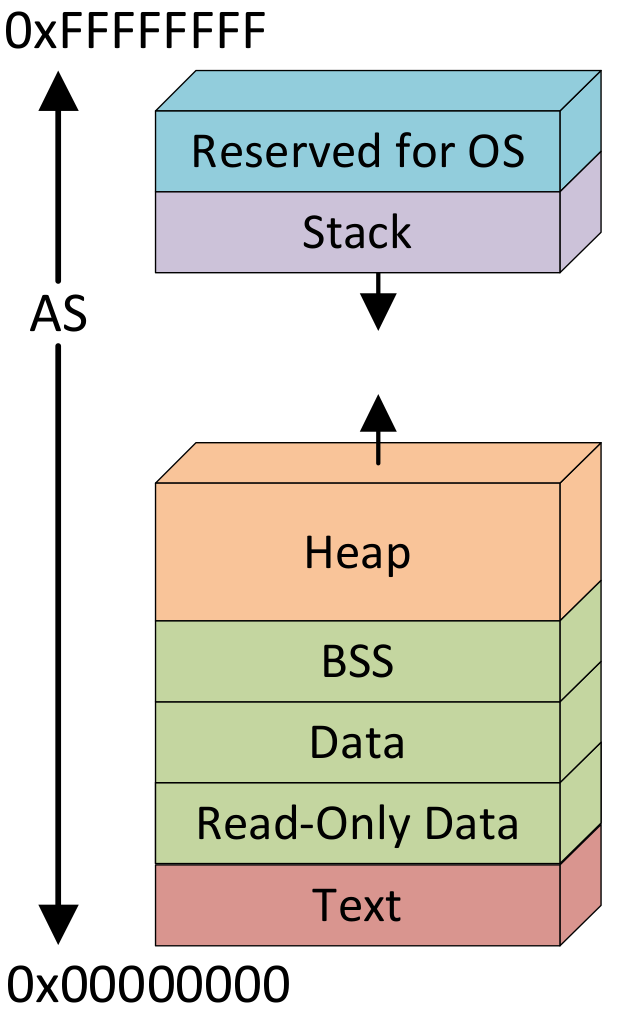
\includegraphics[width=0.2\textwidth]{AddressSpaceLayoutComplex}\end{figure}

\begin{summary}
	\textbf{Processes}: recipe vs. cooking = program vs. process
	\begin{itemize}
		\item processes = resource container for OS
		\item process feels alone (has own CPU and memory) 
		\item OS implements multiprogramming through rapid process switching
	\end{itemize}
\end{summary}
